\chapter{파동함수, 밀도 행렬, 그리고 국소성}

\lectureoverview{벨의 정리를 뒤로 미루는 데에는 한 가지 중요한 이유가 있다. 벨의 정리가 무엇을 금지하는지 묻기 전에, 얽힘이 무엇인지 정확히 밝혀야 한다. 두 부분계 상태가 앨리스의 상태 하나와 밥의 상태 하나의 곱으로 인수분해될 수 없을 때, 그 상태는 얽혀 있다. 파동함수는 이 기준을 구체적으로 보여 주고, 상관관계는 그 결과를 드러내며, 싱글렛은 결정적인 예를 제공한다. 이어서 축약 밀도 행렬은 얽힌 전체의 한 부분을 완전히 기술하는 국소적 설명이 된다. 이 형식론을 갖추고 나면 측정은 얽힘을 만드는 상호작용으로 나타나고, 계--관측자 경계는 예측을 바꾸지 않은 채 옮길 수 있으며, 얽힘과 국소성 사이의 겉보기 긴장은 명확히 진술할 수 있다. 멀리 떨어진 곳에서의 선택은 조건부 상관관계를 바꾸지만, 신호 전달에 쓸 수 있는 무조건부 통계는 바꾸지 않는다.}

\section{얽힘의 실제 의미}

곧바로 벨의 정리로 넘어가고 싶을 수 있다. 그 정리는 아름답지만, 정리가 시험하는 구조와 그 의미를 떼어 놓을 수는 없다. 따라서 더 시급한 질문은 아직 양자역학이 벨 부등식을 위반하는지가 아니라, 얽힌 상태가 복합계에 대해 무엇을 말해 주는가이다.

얽힌 두 계가 \emph{하나의 상태를 공유한다}고 흔히 말한다. 하지만 이 표현은 어떤 구별도 해 주지 않는다. 얽혀 있든 아니든 모든 복합계에는 상태가 있다. 구별의 기준은 인수분해 가능성이다. \(A\)와 \(B\)의 힐베르트 공간이 \(\mathcal H_A\)와 \(\mathcal H_B\)라면, 두 계의 쌍은 다음 공간에 속한다.
\begin{equation}
\mathcal H_{AB}=\mathcal H_A\otimes\mathcal H_B.
\end{equation}
순수 상태가 곱 상태라는 것은 다음과 같이 쓸 수 있다는 뜻이다.
\begin{equation}
\ket{\Psi}_{AB}=\ket{\psi}_A\otimes\ket{\phi}_B.
\label{eq:l7-product-state}
\end{equation}
이처럼 인수들의 쌍으로 쓸 수 없다면, \(\ket{\Psi}_{AB}\)는 얽힌 상태다.

\begin{classroomqa}
\audiencequestion{얽힘은 두 계가 하나의 상태 벡터에 함께 들어 있다는 뜻일 뿐인가요?}
\lecturerresponse{아니다. 곱 상태도 두 계 전체의 힐베르트 공간에 속한다. 얽힘은 더 강한, 기저 선택과 무관한 명제다. 즉 전체의 벡터를 앨리스의 벡터 하나와 밥의 벡터 하나의 곱으로 쓸 수 없다는 뜻이다.}
\end{classroomqa}

\begin{classroomqa}
\audiencequestion{기저를 영리하게 바꾸면 얽힌 상태를 곱 상태로 바꿀 수 있나요?}
\lecturerresponse{국소적인 기저 변환이라면 불가능하다. 즉 앨리스의 기저를 하나 바꾸고 밥의 기저를 따로 바꾸는 경우를 말한다. 국소 기저 변환은 각 인수의 좌표를 바꾸지만 상태의 인수분해 가능성은 바꾸지 않는다. 두 계의 결합 힐베르트 공간에서 완전히 임의적인 기저를 택하면 텐서곱 구조를 감출 수는 있지만, 어떤 물리적 자유도가 앨리스와 밥에 속하는지는 달라지지 않는다.}
\end{classroomqa}

\section{힐베르트 공간의 좌표로서의 파동함수}

\emph{파동함수}라는 말은 그 수학적 정의에 포함되지 않는 역사적 이미지를 불러온다. 파동함수는 선택한 기저에서 상태 벡터를 좌표로 나타낸 것이다. 가환 관측량의 완비 집합이 다음과 같은 동시 고유벡터를 갖는다고 하자.
\begin{equation}
\ket{a,b,c,\ldots}.
\end{equation}
기저의 모든 벡터를 구별할 수 있도록 표지들이 완비적이어야 한다. 그러면
\begin{align}
\ket{\Psi}
&=\sum_{a,b,c,\ldots}
\ket{a,b,c,\ldots}
\braket{a,b,c,\ldots}{\Psi} \\
&=\sum_{a,b,c,\ldots}
\psi(a,b,c,\ldots)\ket{a,b,c,\ldots},
\label{eq:l7-wavefunction-expansion}
\end{align}
여기서
\begin{equation}
\psi(a,b,c,\ldots)
=\braket{a,b,c,\ldots}{\Psi}.
\label{eq:l7-wavefunction-definition}
\end{equation}
표지가 연속적이면 이에 대응하는 합은 적분으로 바뀐다.

\begin{figure}[htbp]\centering
\includegraphics[width=0.88\textwidth]{lecture_07_figure_01.png}\caption{완비 기저에서 상태를 나타내는 계수들의 집합으로서의 파동함수.}\lectureframe{00:07:00}\end{figure}

3차원 공간의 입자에서는 가환 표지로 \(x,y,z\)를 택할 수 있고,
\begin{equation}
\psi(x,y,z)=\braket{x,y,z}{\Psi}
\end{equation}는 Schr\"odinger의 익숙한 위치 공간 파동함수다. \(\sigma_z\) 기저에서 스핀 하나의 파동함수는 다음 두 성분뿐이다.
\begin{equation}
\psi(u)=\braket{u}{\Psi},
\qquad
\psi(d)=\braket{d}{\Psi}.
\end{equation}
스핀 두 개에는 표지가 두 개 필요하다.
\begin{equation}
\Psi(a,b)=\braket{a,b}{\Psi},
\qquad
a,b\in\{u,d\}.
\label{eq:l7-two-spin-wavefunction}
\end{equation}
이 정의 어디에도 공간 속에 실제 파동이 있어야 한다는 요구는 없다.

\begin{classroomqa}
\audiencequestion{파동함수의 기저를 바꾸면 푸리에 변환을 하는 건가요?}
\lecturerresponse{푸리에 변환은 위치 표현과 운동량 표현 사이의 특정한 기저 변환이다. 더 일반적으로, 모든 정규직교 기저 변환은 좌표에 대한 유니터리 변환이다. \(\sigma_z\) 기저에서 \(\sigma_x\) 기저로 옮기는 것은 푸리에 변환과 비슷하지만, 위치--운동량 적분 변환이 아니라 유한 차원 유니터리 행렬을 이용한다.}
\end{classroomqa}

\begin{classroomqa}
\audiencequestion{기저를 바꾸면 파동함수가 달라지는데, 물리적 상태도 바뀐 건가요?}
\lecturerresponse{아니다. 켓 \(\ket{\Psi}\)은 추상적인 상태다. 수 \(\psi(a,b,c,\ldots)\)는 선택한 기저에서 그 상태를 나타내는 좌표다. 좌표를 바꾸면 이 수들은 달라지지만 벡터와 모든 물리적 예측은 그대로다.}
\end{classroomqa}

\section{성분으로 나타낸 기댓값}

밀도 행렬을 도입하기 전에 기댓값의 성분 구조를 드러내 보자. \(L\)를 관측량이라 하고, 행렬 원소를 다음과 같이 두자.
\begin{equation}
L_{a'a}=\bra{a'}L\ket{a}.
\label{eq:l7-matrix-elements}
\end{equation}
\(\ket{\Psi}=\sum_a\psi(a)\ket{a}\)라면,
\begin{align}
\expect{L}
&=\bra{\Psi}L\ket{\Psi} \\
&=\sum_{a',a}
\psi^*(a')\bra{a'}L\ket{a}\psi(a) \\
&=\sum_{a',a}\psi^*(a')L_{a'a}\psi(a).
\label{eq:l7-expectation-components}
\end{align}

\begin{figure}[htbp]\centering
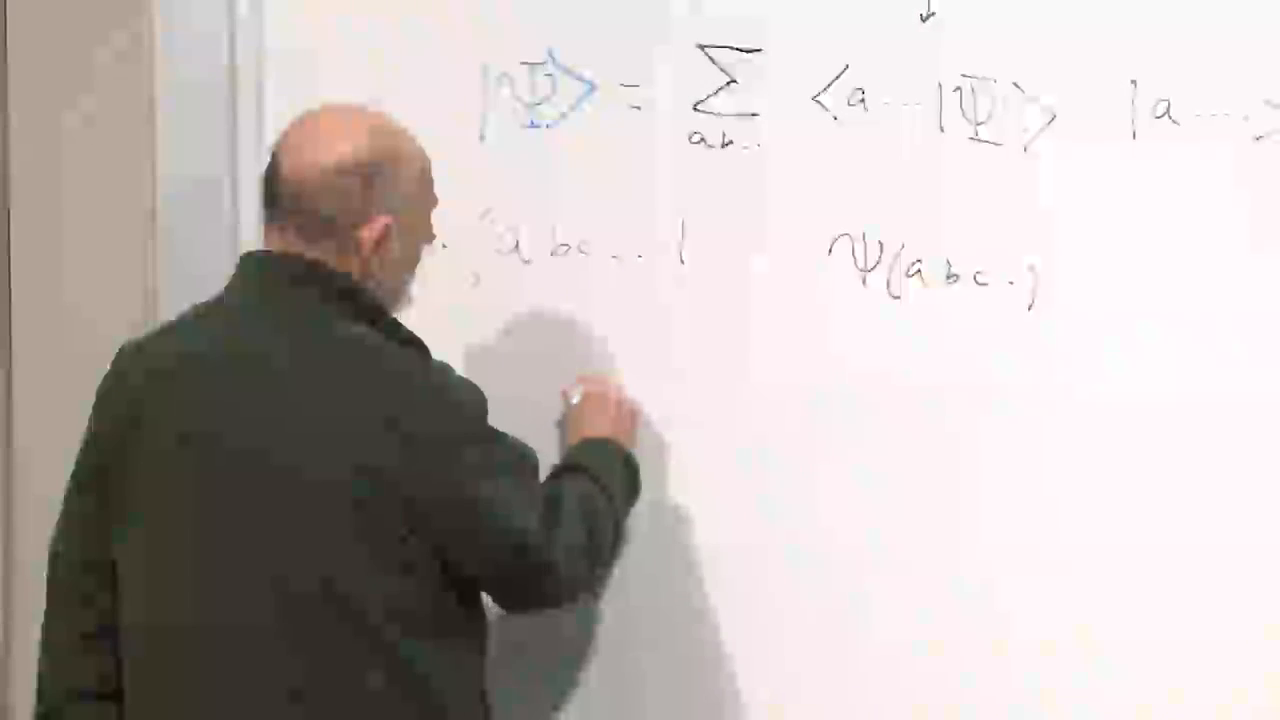
\includegraphics[width=0.88\textwidth]{lecture_07_figure_02.png}\caption{파동함수 계수와 행렬 원소로 전개한 기댓값의 샌드위치 표현.}\lectureframe{00:14:08}\end{figure}

이제 계를 앨리스의 부분과 밥의 부분으로 나누자. 앨리스의 완비 기저 표지를 \(a\), 밥의 완비 기저 표지를 \(b\)라 하자.
\begin{equation}
\ket{\Psi}_{AB}
=\sum_{a,b}\Psi(a,b)\ket{a,b}.
\label{eq:l7-composite-expansion}
\end{equation}
앨리스에만 속하는 관측량은 복합 공간에서 다음 연산자로 나타낸다.
\begin{equation}
L_A=L\otimes I_B,
\end{equation}
따라서 그 행렬 원소는
\begin{equation}
\bra{a',b'}L_A\ket{a,b}
=L_{a'a}\delta_{b'b}.
\label{eq:l7-alice-local-matrix}
\end{equation}
마찬가지로 밥에 국소적인 관측량은 다음 형태다.
\begin{equation}
M_B=I_A\otimes M,
\qquad
\bra{a',b'}M_B\ket{a,b}
=\delta_{a'a}M_{b'b}.
\label{eq:l7-bob-local-matrix}
\end{equation}
건드리지 않는 인수에 항등 연산자가 들어간다는 것은 앨리스의 연산은 앨리스에, 밥의 연산은 밥에 작용한다는 수학적 표현이다.

식 ~\eqref{eq:l7-alice-local-matrix}를 기댓값에 대입하면 다음을 얻는다.
\begin{equation}
\expect{L_A}
=\sum_{a',a,b}
\Psi^*(a',b)L_{a'a}\Psi(a,b).
\label{eq:l7-local-expectation}
\end{equation}
이 식에는 이미 축약 밀도 행렬이 들어 있다. 인수분해가 어떤 결과를 낳는지 먼저 살펴본 뒤 이 식을 재구성하겠다.

\begin{classroomqa}
\audiencequestion{식 ~\eqref{eq:l7-local-expectation}에서 밥의 표지는 왜 하나만 남나요?}
\lecturerresponse{밥의 공간에 대한 항등 연산자는 \(\delta_{b'b}\)를 준다. 이 항은 밥 쪽의 브라 표지와 켓 표지를 같게 하므로, \(b',b\)에 대한 이중 합이 \(b\)에 대한 단일 합으로 줄어든다.}
\end{classroomqa}

\begin{classroomqa}
\audiencequestion{앨리스는 밥이 어떤 기저를 쓰는지 알아야 하나요?}
\lecturerresponse{아니다. 어떤 물리적 예측도 밥의 기저에 의존하지 않는다. 밥의 완비 기저에 대한 합은 항등 연산자의 분해다. 밥의 기저를 바꾸면 개별 성분 \(\Psi(a,b)\)은 달라지지만 앨리스의 기댓값은 달라지지 않는다.}
\end{classroomqa}

\section{곱 상태와 상관관계}

곱 상태에서는 두 계의 파동함수가 인수분해된다.
\begin{equation}
\Psi(a,b)=\psi_A(a)\phi_B(b).
\label{eq:l7-wavefunction-factorization}
\end{equation}
이를 식 ~\eqref{eq:l7-local-expectation}에 대입하자.
\begin{align}
\expect{L_A}
&=\sum_{a',a,b}
\psi_A^*(a')\phi_B^*(b)
L_{a'a}
\psi_A(a)\phi_B(b) \\
&=\left[
\sum_{a',a}\psi_A^*(a')L_{a'a}\psi_A(a)
\right]
\left[
\sum_b|\phi_B(b)|^2
\right] \\
&=\bra{\psi_A}L\ket{\psi_A}.
\label{eq:l7-product-local-expectation}
\end{align}
밥 쪽 인수의 정규화 때문에 그 인수는 1이 된다. 따라서 앨리스의 국소 통계는 밥의 계를 애초에 도입하지 않았을 때와 정확히 같다.

\begin{figure}[htbp]\centering
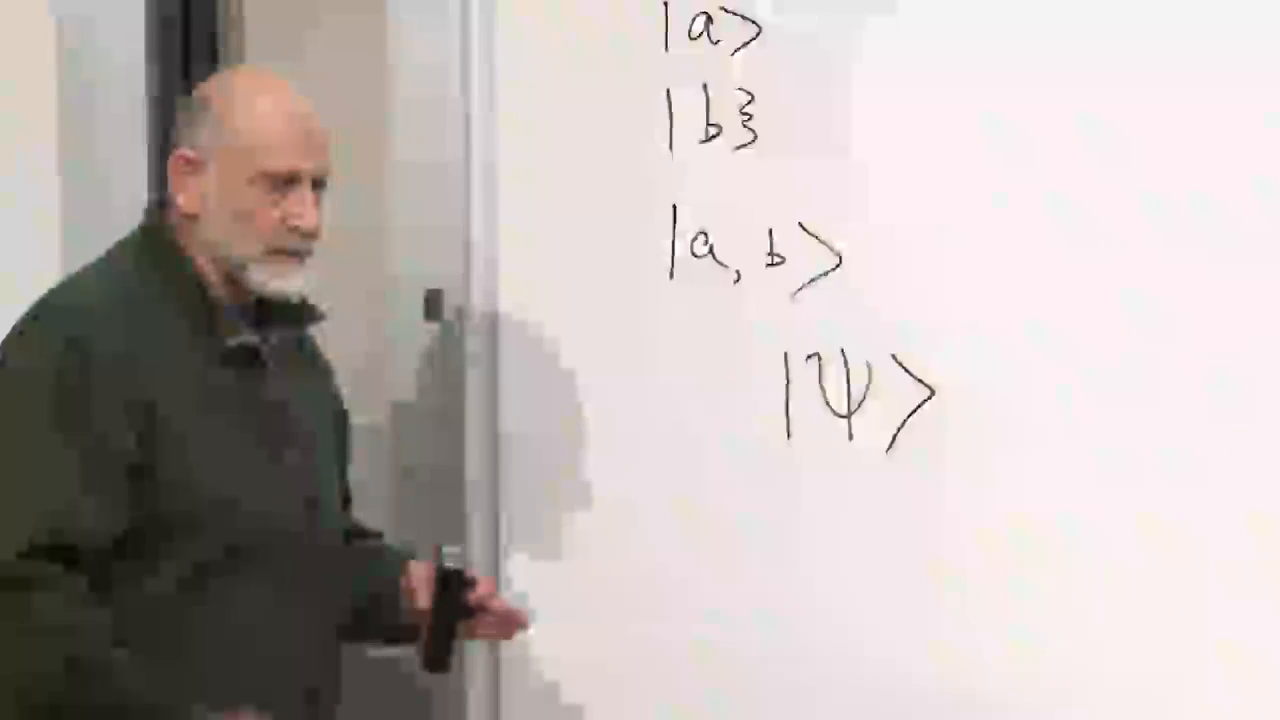
\includegraphics[width=0.88\textwidth]{lecture_07_figure_03.png}\caption{두 계의 파동함수의 인수분해와 이에 따른 국소 기댓값의 분리.}\lectureframe{00:29:18}\end{figure}

Alice의 한 관측가능량과 Bob의 한 관측가능량의 곱은 행렬 원소가 다음과 같다.
\begin{equation}
\bra{a',b'}L_A M_B\ket{a,b}
=L_{a'a}M_{b'b}.
\end{equation}
곱 상태에서는 기댓값이 다음과 같이 인수분해된다.
\begin{equation}
\expect{L_A M_B}
=\expect{L_A}\expect{M_B}.
\label{eq:l7-product-correlation-factorization}
\end{equation}
따라서 연결 상관관계를 다음과 같이 정의하는 것이 자연스럽다.
\begin{equation}
C(L,M)
=\expect{L_A M_B}
-\expect{L_A}\expect{M_B}.
\label{eq:l7-connected-correlation}
\end{equation}
모든 곱 상태에서 모든 국소 관측가능량 쌍에 대해 \(C(L,M)=0\)이다. 반대로 순수한 이분계 상태가 얽혀 있으면 연결 상관관계가 0이 아닌 국소 관측가능량 쌍이 적어도 하나 존재한다.

\begin{classroomqa}
\audiencequestion{\(L_A M_B\)는 밥을 먼저 측정하고 앨리스를 나중에 측정한다는 뜻인가요?}
\lecturerresponse{아니다. 연산자는 상태 벡터에 작용하고, 측정은 측정 장치가 수행한다. 곱의 뜻은 \(M_B\)가 작용한 다음 \(L_A\)가 작용한다는 것이다. 두 연산자는 서로 다른 텐서 인수에 작용하므로 \([L_A,M_B]=0\)이고, 따라서 수학적 순서는 중요하지 않다. 결합 기댓값을 추정하기 위한 실험실 절차는 별개의 문제다.}
\end{classroomqa}

\begin{classroomqa}
\audiencequestion{선택한 상관관계가 사라져도 상태가 얽혀 있을 수 있나요?}
\lecturerresponse{물론입니다. \(C(L,M)\)이 사라진다는 것은 이 특정 관측가능량 쌍에 상관관계가 없다는 뜻일 뿐입니다. 순수 상태가 인수분해되는지 확인하려면 모든 국소 교차 상관관계가 인수분해되어야 합니다. 부분 상관관계가 어떤 단일 수치로 간단히 나타나는 부분 얽힘을 뜻하는 것도 아닙니다. 그 정보는 축약 밀도 행렬의 전체 스펙트럼에 담겨 있습니다.}
\end{classroomqa}

\begin{classroomqa}
\audiencequestion{상관관계가 있는 상태는 모두 얽힌 상태인가요?}
\lecturerresponse{여기서 다루는 순수 상태에서는 인수분해되지 않는 상관관계가 얽힘을 드러낸다. 혼합 상태에서는 고전적 상관관계만으로도 \(C(L,M)\neq0\)가 성립할 수 있다. 따라서 뒤에서 다룰 밀도 행렬 기준에는 전체 상태가 순수하다고 알려져 있는지에 따라 조건을 붙여야 한다.}
\end{classroomqa}

\section{싱글렛: 부분은 불확정이지만 전체는 확정된 상태}

\(\boldsymbol{\sigma}\)가 밥의 스핀에, \(\boldsymbol{\tau}\)가 앨리스의 스핀에 작용한다고 하자. 두 스핀의 싱글렛 상태는 다음과 같다.
\begin{equation}
\ket{S}
=\frac{1}{\sqrt2}
\left(\ket{u d}-\ket{d u}\right),
\label{eq:l7-singlet}
\end{equation}
첫 번째 자리는 밥, 두 번째 자리는 앨리스를 나타낸다. 어느 스핀도 \(z\) 성분이 확정되어 있지 않다.
\begin{equation}
\expect{\sigma_z}=0,
\qquad
\expect{\tau_z}=0.
\label{eq:l7-singlet-local-z}
\end{equation}
하지만 두 성분의 곱은 확정되어 있다.
\begin{equation}
\expect{\sigma_z\tau_z}=-1.
\label{eq:l7-singlet-product-z}
\end{equation}
모든 \(z\) 측정에서 결과는 서로 반대다.

회전 대칭성 때문에 이 명제는 방향에 의존하지 않는다. 임의의 단위 벡터 \(\mathbf n\)에 대해
\begin{equation}
\expect{\boldsymbol{\sigma}\cdot\mathbf n}
=\expect{\boldsymbol{\tau}\cdot\mathbf n}=0,
\qquad
\expect{
(\boldsymbol{\sigma}\cdot\mathbf n)
(\boldsymbol{\tau}\cdot\mathbf n)
}=-1.
\label{eq:l7-singlet-any-axis}
\end{equation}
더 일반적으로,
\begin{equation}
\expect{\sigma_i\tau_j}=-\delta_{ij}.
\label{eq:l7-singlet-correlation-tensor}
\end{equation}
각 부분계는 완전히 비편극 상태인 반면, 같은 축에서 측정한 결과는 완벽하게 반상관되어 있다.

\begin{figure}[htbp]
\centering
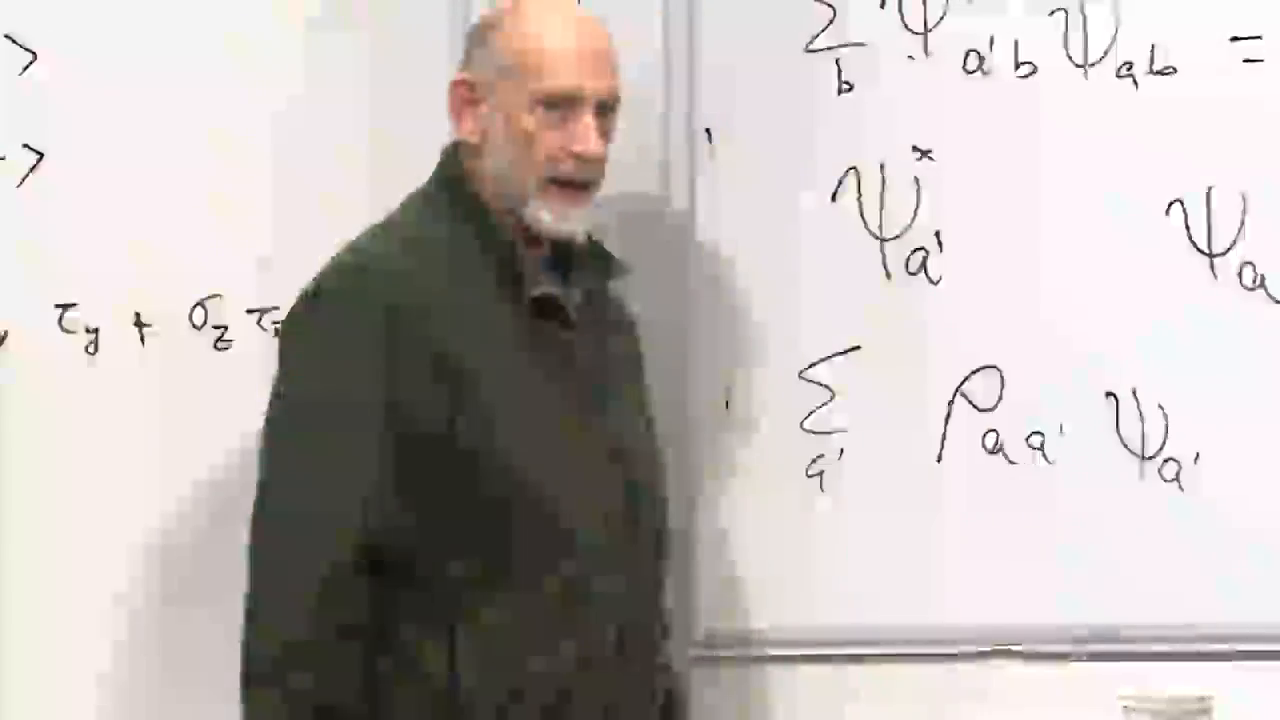
\includegraphics[width=0.88\textwidth]{lecture_07_figure_04.png}
\caption{싱글렛에서는 각 국소 스핀의 평균이 사라지고, 같은 성분끼리 곱한 값은 \(-1\)이다.}
\lectureframe{00:38:28}
\end{figure}

이것이 얽힘이 만들어내는 특징적인 역전이다. 고립된 스핀이 순수 상태에 있으면 스핀이 확정되는 방향이 하나 존재한다. 싱글렛에서는 어느 방향에서도 어느 한쪽의 국소 스핀조차 확정되지 않는다. 그런데도 복합계의 상태는 순수하며 완전히 특정되어 있다. 전체에 대해 양자역학이 허용하는 만큼의 정보를 알고 있어도 각 부분에 순수 상태를 부여할 수는 없다.

\begin{classroomqa}
\audiencequestion{전체의 상태를 정확히 알고 있는데, 왜 각 스핀의 확정된 상태를 추론할 수 없나요?}
\lecturerresponse{싱글렛은 곱 상태가 아니기 때문이다. 그 계수는 밥의 진폭 하나와 앨리스의 진폭 하나의 곱으로 분리되지 않는다. 정보는 서로 독립적으로 존재하는 두 국소 파동함수에 있는 것이 아니라 두 부분계 사이의 관계에 담겨 있다.}
\end{classroomqa}

\begin{classroomqa}
\audiencequestion{\(\sigma_z\) 같은 연산자 자체가 스핀의 가능한 상태인가요?}
\lecturerresponse{아니다. 상태는 벡터이거나, 더 일반적으로 밀도 연산자다. \(\sigma_z\)는 상태에 작용하는 관측량이다. \(\sigma_z\)의 고유벡터는 \(z\) 성분이 확정된 상태지만, 관측량과 그 고유벡터는 서로 다른 종류의 대상이다.}
\end{classroomqa}

\begin{classroomqa}
\audiencequestion{\(\sigma_z\tau_z\ket{S}=-\ket{S}\)라고 쓸 때 측정을 수행한 건가요?}
\lecturerresponse{아니다. 이 식은 연산자가 벡터에 어떻게 작용하는지를 나타낸다. 해당 결합 관측량을 측정하면 반드시 \(-1\)을 얻는다는 뜻이지만, 고유값 방정식을 썼다고 해서 검출기가 도입된 것은 아니다.}
\end{classroomqa}

\begin{classroomqa}
\audiencequestion{얽힌 두 스핀은 상관관계가 부분적일 수도 있나요?}
\lecturerresponse{그렇다. 완벽한 반상관관계는 같은 축에 대해 싱글렛이 갖는 특별한 성질이다. 다른 얽힌 상태는 더 약한 상관관계를 가질 수 있고, 싱글렛에서도 두 축이 다르면 \(-\mathbf a\cdot\mathbf b\)이지 \(-1\)는 아니다. 얽힘의 기준은 인수분해 불가능성이지, 선택한 모든 측정에서 완벽하게 일치하거나 불일치하는지가 아니다.}
\end{classroomqa}

\section{에너지 완화에 의한 싱글렛 준비}

회전 불변인 두 스핀 연산자는
\begin{equation}
\boldsymbol{\sigma}\cdot\boldsymbol{\tau}
=\sigma_x\tau_x+\sigma_y\tau_y+\sigma_z\tau_z
\label{eq:l7-spin-dot-spin}
\end{equation}
4차원 상태 공간을 구성한다. 싱글렛에서는
\begin{equation}
(\boldsymbol{\sigma}\cdot\boldsymbol{\tau})\ket{S}
=-3\ket{S},
\label{eq:l7-singlet-dot-eigenvalue}
\end{equation}
세 개의 트립렛 상태는 각각 고유값 \(+1\)를 갖는다.

\begin{figure}[htbp]\centering
\includegraphics[width=0.88\textwidth]{lecture_07_figure_05.png}\caption{회전 불변 결합 \(\boldsymbol{\sigma}\cdot\boldsymbol{\tau}\)와 싱글렛 및 트립렛 부분공간을 구분하는 역할.}\lectureframe{00:52:33}\end{figure}

상호작용 해밀토니안에 다음 항이 있다고 하자.
\begin{equation}
H_{\mathrm{int}}
=J\,\boldsymbol{\sigma}\cdot\boldsymbol{\tau}.
\label{eq:l7-exchange-hamiltonian}
\end{equation}
반강자성 결합 \(J>0\)의 경우 싱글렛은 트립렛보다 다음만큼 에너지가 낮다.
\begin{equation}
\Delta E=4J.
\end{equation}
두 스핀을 가까이 두고, 광자나 포논 또는 다른 여기 상태를 방출하며 고에너지 성분이 붕괴하도록 하면, 두 스핀은 싱글렛을 향해 완화된다. 두 스핀 사이의 분리가 제어되지 않는 스핀 회전을 일으키지 않고 에너지 간격을 지나치게 급격히 닫지 않는다면, 두 스핀을 분리한 뒤에도 결합 상태를 보존할 수 있다.

같은 에너지 논리는 원자 계에서도 나타난다. 예를 들어 포지트로늄에서는 전자와 양전자의 스핀 결합이 싱글렛 배치와 트립렛 배치 사이의 에너지 간격을 만든다. 에너지 차이는 \(E=mc^2\)에 따라 질량 차이이기도 하지만, 분광학에서는 보통 이 간격을 에너지나 진동수로 나타낸다.

\begin{classroomqa}
\audiencequestion{두 스핀이 상호작용하면 싱글렛은 언제나 바닥 상태인가요?}
\lecturerresponse{아니다. 식 ~\eqref{eq:l7-exchange-hamiltonian}에서 \(J>0\)인 경우에 바닥 상태다. 부호를 반대로 하면 트립렛이 더 낮은 에너지를 갖는다. 준비 과정에 대한 설명은 단지 스핀이 두 개 있다는 사실이 아니라 실제 상호작용과 에너지 준위 순서에 달려 있다.}
\end{classroomqa}

\begin{classroomqa}
\audiencequestion{\(\boldsymbol{\sigma}\cdot\boldsymbol{\tau}\)는 세 성분을 각각 측정해서 구할 수 있나요?}
\lecturerresponse{한 쌍에서 세 국소 스핀 성분을 동시에 측정해서는 안 된다. \(\sigma_x,\sigma_y,\sigma_z\)는 서로 양립하지 않고, 세 \(\tau\) 성분도 서로 양립하지 않는다. \(x,y,z\) 방향으로 측정한 세 부분 앙상블을 이용해 기댓값을 재구성할 수도 있고, 적절한 결합 측정 장치로 싱글렛--트립렛 관측량을 직접 측정할 수도 있다.}
\end{classroomqa}

\begin{classroomqa}
\audiencequestion{스핀을 분리한 뒤에도 얽힘을 유지하려면 계속 상호작용해야 하나요?}
\lecturerresponse{아니다. 상태를 준비하거나 바꾸려면 상호작용이 필요하지만, 싱글렛을 일단 준비하고 나면 입자 사이에 지속적인 힘이 작용하지 않아도 유니터리 시간 발전으로 얽힘을 보존할 수 있다. 국소 자기장은 두 인수를 회전시킬 수 있지만, 국소 유니터리 회전만으로 얽힘이 파괴되지는 않는다.}
\end{classroomqa}

\section{축약 밀도 행렬}

앨리스의 국소 기댓값으로 돌아가자.
\begin{equation}
\expect{L_A}
=\sum_{a',a,b}
\Psi^*(a',b)L_{a'a}\Psi(a,b).
\end{equation}
\(L\)에 속하지 않는 인수들을 묶으면
\begin{equation}
\expect{L_A}
=\sum_{a',a}
\left[
\sum_b\Psi(a,b)\Psi^*(a',b)
\right]L_{a'a}.
\label{eq:l7-regrouped-expectation}
\end{equation}
대괄호 안의 식이 앨리스의 축약 밀도 행렬이다.
\begin{equation}
(\rho_A)_{aa'}
=\sum_b\Psi(a,b)\Psi^*(a',b).
\label{eq:l7-reduced-density-components}
\end{equation}
기저에 무관한 표기로는
\begin{equation}
\rho_A
=\operatorname{Tr}_B\ket{\Psi}\bra{\Psi},
\label{eq:l7-partial-trace}
\end{equation}
앨리스에 국소적인 모든 기댓값은 다음과 같다.
\begin{equation}
\expect{L_A}
=\operatorname{Tr}_A(\rho_A L).
\label{eq:l7-density-expectation}
\end{equation}

\begin{figure}[htbp]\centering
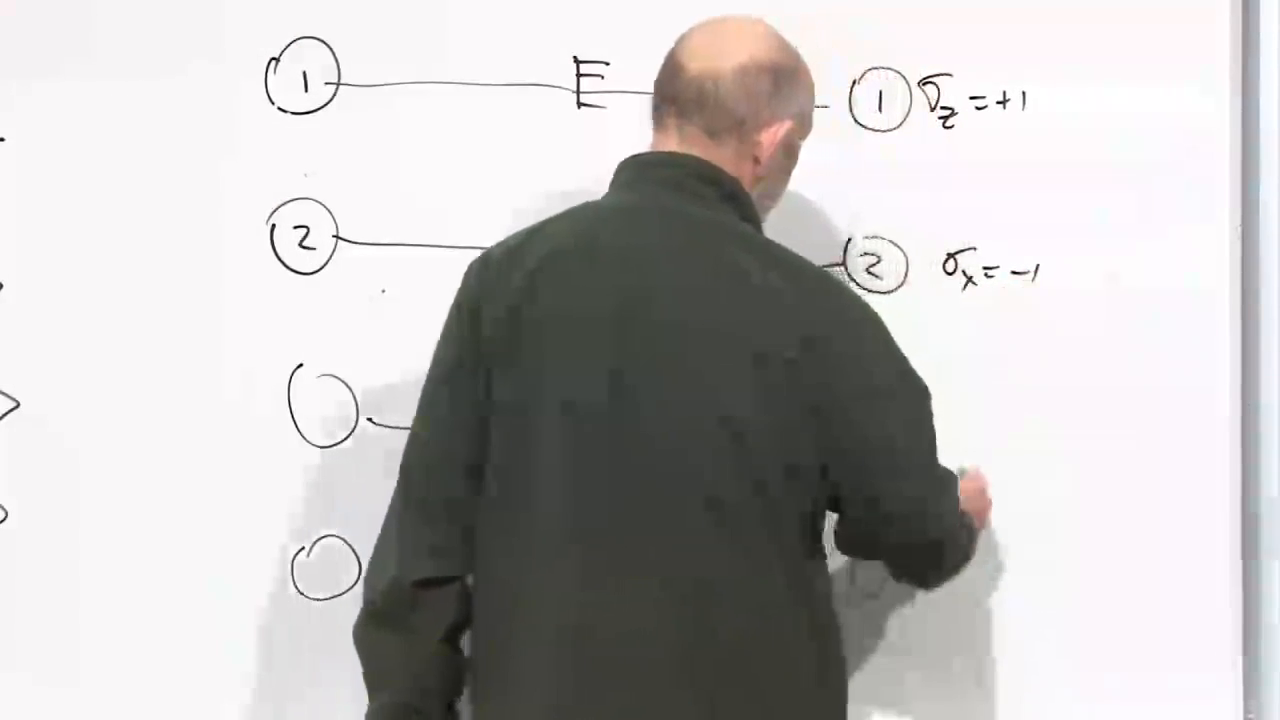
\includegraphics[width=0.88\textwidth]{lecture_07_figure_06.png}\caption{밥의 기저 표지에 대해 결합 진폭을 합산해 구한 앨리스의 밀도 행렬.}\lectureframe{01:02:33}\end{figure}

축약 밀도 행렬은 에르미트이고 양의 정부호이며 정규화되어 있다.
\begin{equation}
\rho_A^\dagger=\rho_A,
\qquad
\bra{\chi}\rho_A\ket{\chi}\geq0,
\qquad
\operatorname{Tr}\rho_A=1.
\label{eq:l7-density-properties}
\end{equation}
앨리스에게 국한된 모든 측정에 필요한 정보가 정확히 여기에 담겨 있다. 두 전역 상태가 같은 \(\rho_A\)를 만든다면, 앨리스 혼자 하는 어떤 실험으로도 두 상태를 구별할 수 없다.

\begin{classroomqa}
\audiencequestion{앨리스는 밀도 행렬을 하나의 관측량처럼 측정하나요?}
\lecturerresponse{한 번의 측정으로는 아니다. 밀도 행렬은 모든 국소 측정 확률을 계산하는 데 쓰이는 대상이다. 똑같이 준비된 계가 많이 주어지면 앨리스는 토모그래피로 밀도 행렬을 재구성할 수 있다. 충분한 관측량 집합을 측정하고 그 기댓값에서 행렬을 추론하는 것이다.}
\end{classroomqa}

\begin{classroomqa}
\audiencequestion{밥의 상태 하나를 고르지 않고 왜 밥에 대해 합산하나요?}
\lecturerresponse{앨리스는 밥의 측정 결과에 대한 정보를 갖고 있지 않기 때문이다. 부분 추적은 밥의 완비 기저에 대해 합산하여 조건을 걸지 않은 국소 상태를 준다. 대신 밥의 특정 측정 결과 하나를 선택하면 조건부 상태가 나오는데, 이는 다른 연산이며 그 결과를 알아야 한다.}
\end{classroomqa}

곱 상태 \(\Psi(a,b)=\psi_A(a)\phi_B(b)\)에서는
\begin{align}
(\rho_A)_{aa'}
&=\sum_b
\psi_A(a)\phi_B(b)
\psi_A^*(a')\phi_B^*(b) \\
&=\psi_A(a)\psi_A^*(a')
\sum_b|\phi_B(b)|^2 \\
&=\psi_A(a)\psi_A^*(a').
\end{align}
따라서
\begin{equation}
\rho_A=\ket{\psi_A}\bra{\psi_A}.
\label{eq:l7-pure-projector}
\end{equation}
이것은 계수 1인 사영 연산자다. 이를 \(\ket{\psi_A}\)에 작용시키면
\begin{equation}
\rho_A\ket{\psi_A}
=\ket{\psi_A}\braket{\psi_A}{\psi_A}
=\ket{\psi_A},
\label{eq:l7-density-on-state}
\end{equation}
한편 \(\ket{\psi_A}\)에 직교하는 임의의 \(\ket{\chi}\)에 대해서는
\begin{equation}
\rho_A\ket{\chi}
=\ket{\psi_A}\braket{\psi_A}{\chi}
=0.
\label{eq:l7-density-on-orthogonal}
\end{equation}

\begin{figure}[htbp]\centering
\includegraphics[width=0.88\textwidth]{lecture_07_figure_07.png}\caption{곱 상태의 밀도 행렬이 사영 연산자로 작용하는 모습: \(\ket{\psi_A}\) 방향의 고유값은 \(1\)이고, 직교 벡터의 고유값은 \(0\)이다.}\lectureframe{01:09:43}\end{figure}

\section{밀도 행렬의 스펙트럼과 얽힘}

\(\rho_A\)의 고윳값은 모두 음이 아니며 합은 1이다. 전체 계가 순수 상태이면 다음과 같다.
\begin{itemize}
\item 영이 아닌 고윳값이 정확히 하나이고 그 값이 \(1\)이면 상태는 곱 상태이다.
\item 영이 아닌 고윳값이 둘 이상이면 상태는 얽혀 있다.
\item 가능한 국소 지지공간 전체에 걸쳐 고윳값이 같으면 최대 얽힘 상태이다.
\end{itemize}
Schmidt 분해를 이용하면 이 내용을 가장 명확하게 볼 수 있다.
\begin{equation}
\begin{aligned}
\ket{\Psi}_{AB}
&=\sum_{r=1}^{R}\sqrt{\lambda_r}
\ket{r}_A\ket{r}_B,\\
\lambda_r&\geq0,
\qquad
\sum_r\lambda_r=1.
\end{aligned}
\label{eq:l7-schmidt}
\end{equation}
이때 다음이 성립한다.
\begin{equation}
\rho_A=\sum_{r=1}^{R}\lambda_r\ket{r}_A\bra{r}.
\label{eq:l7-schmidt-density}
\end{equation}
Schmidt 계수의 개수 \(R\)는 곱 상태에서 하나이고, 얽힌 순수 상태에서는 하나보다 크다.

싱글렛의 경우,
\begin{equation}
\rho_A
=\operatorname{Tr}_B\ket{S}\bra{S}
=\frac12\ket{u}\bra{u}
+\frac12\ket{d}\bra{d}
=\frac12 I.
\label{eq:l7-singlet-reduced-density}
\end{equation}
고윳값은 다음과 같다.
\begin{equation}
\operatorname{spec}(\rho_A)
=\left\{\frac12,\frac12\right\}.
\end{equation}
두 스핀의 상태가 순수한데도 앨리스의 국소 상태는 최대 혼합 상태다.

스펙트럼은 정량적 척도를 시사한다. 폰 노이만 엔트로피는
\begin{equation}
S(\rho_A)
=-\operatorname{Tr}(\rho_A\log\rho_A)
=-\sum_r\lambda_r\log\lambda_r
\label{eq:l7-entanglement-entropy}
\end{equation}
곱 순수 상태에서는 사라지고, 최대 얽힘 상태에서는 \(\log d_A\)에 도달한다. 이는 \(d_A\leq d_B\)일 때 성립한다. 엔트로피의 구체적인 활용은 뒤로 미뤄도 된다. 스펙트럼만으로도 핵심적인 구분은 드러난다.

\begin{classroomqa}
\audiencequestion{얽힌 축약 밀도 행렬의 고윳값은 모두 영이 아니어야 하나요?}
\lecturerresponse{아닙니다. 영이 아닌 고윳값이 둘 이상이면 충분합니다. Alice의 힐베르트 공간이 큰 경우 얽힌 상태가 더 낮은 차원의 Schmidt 부분공간만 차지하여 나머지 고윳값은 영일 수 있습니다. 최대 얽힘이란 임의로 고른 일부 고윳값만 같은 상태가 아니라 더 작은 부분계 전체에 걸쳐 고윳값이 같은 상태를 뜻합니다.}
\end{classroomqa}

\begin{classroomqa}
\audiencequestion{혼합된 축약 밀도 행렬만으로 앨리스가 밥과 얽혀 있음을 증명할 수 있나요?}
\lecturerresponse{전체 상태가 순수하다고 알려져 있을 때에만 그렇다. 전역 상태가 혼합 상태라면 일반적인 고전적 혼합 때문에도 국소 상태가 혼합 상태가 될 수 있다. 하지만 순수한 두 부분계 상태에서는 국소 상태의 혼합성이 곧 두 부분계 사이의 얽힘과 동치다.}
\end{classroomqa}

\begin{classroomqa}
\audiencequestion{앨리스 관측량의 모든 모멘트로 확률 분포를 결정할 수 있나요?}
\lecturerresponse{유한 차원 계에서는 연산자 기저의 기댓값으로 \(\rho_A\)를 결정할 수 있고, \(\rho_A\)에서 본 규칙에 따라 모든 국소 측정 결과의 분포를 구할 수 있다. 재구성에는 동일하게 준비된 계의 앙상블이 필요하다. 고립된 한 사건만으로 밀도 행렬을 알아낼 수는 없다.}
\end{classroomqa}

\section{얽힘을 만드는 상호작용으로서의 측정}

앨리스와 밥을 스핀과 측정 장치로 바꾸어 보자. 측정 장치가 준비된 상태 \(\ket{0}_D\)와 작동된 상태 \(\ket{1}_D\)를 갖는다고 하자. 스핀이 위 방향인지 기록하는 이상적 상호작용은 다음과 같이 나타낼 수 있다.
\begin{align}
\ket{u}\ket{0}_D&\longrightarrow\ket{u}\ket{1}_D,\\
\ket{d}\ket{0}_D&\longrightarrow\ket{d}\ket{0}_D.
\label{eq:l7-measurement-basis-map}
\end{align}
검출기는 알려진 준비 상태에서 시작해야 한다. 그렇지 않으면 최종 상태가 분명한 기록이 되지 않는다.

중첩 상태의 시간 발달은 선형성에 따라 정해진다.
\begin{equation}
\left(\alpha\ket{u}+\beta\ket{d}\right)\ket{0}_D
\longrightarrow
\alpha\ket{u}\ket{1}_D
+\beta\ket{d}\ket{0}_D.
\label{eq:l7-measurement-entanglement}
\end{equation}
두 계수 중 어느 하나가 영이 되지 않는 한 최종 상태는 얽혀 있다. 포인터 상태가 스핀과 상관관계를 이루었기 때문에 장치는 정보를 얻었다.

\begin{figure}[htbp]\centering
\includegraphics[width=0.88\textwidth]{lecture_07_figure_08.png}\caption{이상적인 측정은 스핀의 각 대안을 서로 다른 포인터 상태와 상관짓고, 그 결과 얽힘을 만든다.}\lectureframe{01:20:20}\end{figure}

스핀만 남기고 검출기를 무시하면, 포인터 기록이 서로 직교한다는 가정 아래 스핀의 축약 상태는 다음과 같다.
\begin{equation}
\rho_{\mathrm{spin}}
=|\alpha|^2\ket{u}\bra{u}
+|\beta|^2\ket{d}\bra{d},
\label{eq:l7-postmeasurement-reduced-state}
\end{equation}
검출기와의 상관관계에 간섭항이 저장되었기 때문에 국소 기술에서는 그 항이 사라졌다.

이제 상보적인 설명 두 가지가 있다. 검출 결과를 읽고 그 기록에 조건을 걸면, 스핀에는 해당 분기가 부여된다. 작동 기록이 있으면 \(\ket{u}\), 없으면 \(\ket{d}\)이다. 이것이 붕괴 설명이다. 검출기와 스핀을 하나의 닫힌 계로 다루면 식 ~\eqref{eq:l7-measurement-entanglement}는 보통의 유니터리 시간 발전이고, 결합 상태에서 어떤 분기도 제거되지 않는다.

\begin{classroomqa}
\audiencequestion{측정은 얽힘과 별개의 현상인가요?}
\lecturerresponse{계--측정 장치 동역학의 수준에서 측정은 신뢰할 수 있는 상관관계를 만드는 상호작용이다. 붕괴는 분명한 기록을 선택한 뒤 사용하는 조건부 기술이다. 그 갱신을 근본적인 것으로 볼지, 선택한 경계에 상대적인 것으로 볼지는 해석의 문제다. 조작적으로 얻는 예측은 서로 일치한다.}
\end{classroomqa}

\begin{classroomqa}
\audiencequestion{이상적인 측정은 왜 스핀 고유상태를 그대로 두나요?}
\lecturerresponse{이 모형에서 요구하는 반복 가능성 때문이다. 입력 상태가 이미 측정하는 관측량의 고유상태라면, 측정 장치는 그 값을 바꾸지 않고 기록해야 한다. 실제 측정은 상태를 파괴할 수 있지만, 그런 경우에는 상호작용을 다른 방식으로 모형화해야 한다.}
\end{classroomqa}

\section{관측자의 위계}

측정 장치를 양자계로 받아들이면 거기서 멈출 만한 자연스러운 이유가 없다. 포인터에서 나온 빛은 눈과 상호작용하고, 눈에서 온 신호는 뇌와 상관관계를 맺으며, 어떤 관측자는 또 다른 관측자에게 관찰될 수 있다. Schr\"odinger의 고양이와 위그너의 친구는 이 중첩 구조를 극적으로 보여 준다.
\begin{equation}
\begin{gathered}
\text{spin}
\longrightarrow
\text{apparatus}
\longrightarrow
\text{cat}\\
\longrightarrow
\text{Schr\"odinger}
\longrightarrow
\text{Wigner}.
\end{gathered}
\label{eq:l7-observer-chain}
\end{equation}
선택한 경계 안에서는 이 연쇄를 유니터리 시간 발전과 점점 커지는 얽힘으로 기술할 수 있다. 경계 밖에서는 측정 결과에 조건을 건 붕괴의 언어를 쓴다.

핵심적인 일관성 조건은 경계를 옮길 수 있어야 한다는 것이다. 고양이가 스핀이 위 방향임을 기록하면 Schr\"odinger는 나중에 고양이가 스핀이 위 방향임을 보았다고 기록해야 하며, 위그너는 Schr\"odinger가 그 이력을 똑같이 기록했다고 기록해야 한다. 양자역학은 객관적 사건이 선언되어야 하는 유일하고 명확한 선을 지정하지 않는다. 고양이와 눈, 뇌는 모두 물리적 자유도로 이루어져 있다. 그중 하나를 양자역학에서 제외하려면 별도의 법칙이 필요하다.

이로 인한 불편함에 대해 파인먼은 실용주의적인 태도를 보였다. 개념적 문제가 너무 커서 문제가 하나 있는지조차 말하기 어려울 수 있지만, 계산 규칙은 계속해서 적용 가능한 모든 실험을 예측한다. 형식론의 목적은 특정 해석을 강요하는 것이 아니라 불편함의 근원을 정확히 드러내는 데 있다. 전체를 완전히 알고 있어도 그 부분들을 순수 상태로 기술할 수 없을 수 있다.

\begin{classroomqa}
\audiencequestion{내가 고양이라면 경계를 나 자신에게 그어야 하나요?}
\lecturerresponse{자신이 알 수 있는 분명한 기록에 대해서는 붕괴 설명을 쓸 수 있다. 당신을 더 큰 고립계에 포함하는 다른 관측자는 얽힌 상태로 기술할 수 있다. 모두가 같은 경계를 그어야 한다는 것이 요구사항은 아니다. 관측자들이 나중에 결과를 비교할 때 모든 기술이 일관된 기록을 내놓아야 한다는 것이 요구사항이다.}
\end{classroomqa}

\begin{classroomqa}
\audiencequestion{객관적 사건은 원자, 고양이, Schr\"odinger, 위그너 중 어디에서 일어나나요?}
\lecturerresponse{유니터리 형식론은 이 위치 중 어느 것도 특별한 경계로 선택하지 않는다. 어쩌면 \emph{일어나다} 같은 일상적인 말을 정확한 의미가 성립하는 범위 너머까지 밀어붙이고 있는지도 모른다. 형식적 도구는 상관관계가 어떻게 전파되는지, 각 관측자가 무엇을 예측할 수 있는지를 알려 준다. 최종 경계를 어떻게 해석할지는 별개의 문제다.}
\end{classroomqa}

\subsection{약한 결합과 불완전한 판독}

식 ~\eqref{eq:l7-measurement-basis-map}의 이상적인 사상은 서로 완벽하게 구별되는 기록을 만든다. 상호작용이 더 약하면 측정 장치의 상태는 부분적으로만 구별될 수 있다.
\begin{equation}
\alpha\ket{u}\ket{D_u}
+\beta\ket{d}\ket{D_d},
\qquad
0<|\braket{D_d}{D_u}|<1.
\label{eq:l7-weak-measurement}
\end{equation}
그러면 측정 장치는 일부 정보만 얻고 얽힘도 불완전하다. 약한 측정 또는 불명확한 측정이 바로 이런 경우다.

이 상황은 이후 단계의 판독이 좋지 않은 경우와 구별해야 한다. 검출기가 이미 스핀과 완전히 상관관계를 맺었는데도 눈, 케이블, 증폭기 또는 뇌가 기록을 제대로 전달하지 못할 수 있다. 첫 번째 경우에는 계--검출기 상호작용이 약하다. 두 번째 경우에는 검출기에 좋은 기록이 존재하지만 이후 정보 전달의 효율이 낮다. 검출 효율은 어느 단계에서든 영향을 받을 수 있으므로, 원인을 따지기 전에 어떤 물리적 결합이 문제인지 확인해야 한다.

\begin{classroomqa}
\audiencequestion{시력이 좋지 않아 포인터가 가리키는 곳이 불확실하다면, 양자 측정은 약한 측정이었나요?}
\lecturerresponse{반드시 그렇지는 않습니다. 스핀은 장치와 강하고 완전하게 상관되어 있었지만, 장치에서 눈으로 또는 눈에서 뇌로 전달되는 과정이 불완전했을 수 있습니다. 진정한 약한 측정이란 처음의 계--장치 결합 자체가 서로 부분적으로만 구별되는 기록을 만들어 낸 경우를 뜻합니다.}
\end{classroomqa}

\section{국소성과 신호 전달 금지}

\emph{원격 작용}이라는 표현에는 조작적으로 정의되는 의미가 있어야 합니다. 보통의 물리학에서 원격 작용은 여기서 관측할 수 있는 것을 바꿉니다. 태양이 사라지고 지구의 운동이 빛이 오는 시간만큼 기다리지 않고 즉시 바뀐다면, 그 변화를 이용해 빛보다 빠르게 정보를 전달할 수 있을 것입니다. 그것이 진정한 비국소 신호 전달입니다.

얽힘은 그런 신호 전달을 허용하지 않습니다. 밥이 크라우스 연산자 \(K_\mu\)로 나타내는 국소 양자 연산을 수행한다고 합시다.
\begin{equation}
\sum_\mu K_\mu^\dagger K_\mu=I_B.
\end{equation}
앨리스가 밥의 측정 결과를 알지 못한다면, 최종 합동 상태는 다음과 같습니다.
\begin{equation}
\rho'_{AB}
=\sum_\mu
(I_A\otimes K_\mu)\rho_{AB}
(I_A\otimes K_\mu^\dagger).
\end{equation}
밥에 대해 부분 추적을 취하면 다음을 얻습니다.
\begin{equation}
\rho'_A
=\operatorname{Tr}_B\rho'_{AB}
=\operatorname{Tr}_B\rho_{AB}
=\rho_A.
\label{eq:l7-no-signaling}
\end{equation}
따라서 조건을 걸지 않은 앨리스의 모든 국소 확률은 밥이 자취 보존 국소 연산 중 무엇을 선택하든 변하지 않습니다.

측정 결과에 조건을 건 상태는 다릅니다. 밥이 측정하여 결과 \(\mu\)를 얻으면, 앨리스는 다음과 같이 상태를 부여할 수 있습니다.
\begin{equation}
\rho_{A|\mu}
=\frac{
\operatorname{Tr}_B\!\left[
(I_A\otimes K_\mu)\rho_{AB}
(I_A\otimes K_\mu^\dagger)
\right]
}{p_\mu}.
\label{eq:l7-conditioned-state}
\end{equation}
그러나 밥이 보통의 신호로 \(\mu\)을 전달하기 전까지 앨리스는 어떤 \(\rho_{A|\mu}\)인지 알 수 없습니다. 메시지가 도착하기 전에는 결과들에 대해 평균을 취해야 합니다.
\begin{equation}
\sum_\mu p_\mu\rho_{A|\mu}=\rho_A.
\label{eq:l7-conditioned-average}
\end{equation}

\begin{classroomqa}
\audiencequestion{밥이 먼저 측정하면 앨리스의 밀도 행렬은 언제 바뀌나요?}
\lecturerresponse{조건을 걸지 않은 앨리스의 밀도 행렬은 바뀌지 않습니다. 밥의 측정 결과가 앨리스에게 전달되면, 앨리스는 그 결과에 대응하는 조건부 밀도 행렬로 바꿔 쓸 수 있습니다. 이 갱신은 새로 알게 된 정보를 반영하며, 고전적 메시지가 도착하기 전에는 이용할 수 없습니다.}
\end{classroomqa}

\begin{classroomqa}
\audiencequestion{밥의 측정은 같은 순간에 앨리스의 상태를 물리적으로 붕괴시키나요?}
\lecturerresponse{해석에 따라 조건부 갱신을 설명하는 방식은 다르지만, 검증 가능한 다음 진술에는 모두 동의합니다. 밥의 정보가 이용 가능해질 때까지 앨리스의 국소 결과 확률은 변하지 않습니다. 제어 가능한 순간적 신호는 생기지 않습니다.}
\end{classroomqa}

번호가 매겨진 여러 줄에 싱글렛 쌍을 많이 배치했다고 합시다. 밥은 한 쌍의 입자에서 \(z\) 방향을, 다른 쌍에서는 \(x\) 방향을, 또 다른 쌍에서는 \(y\) 방향을 측정하는 식으로 진행합니다. 어느 줄에서든 앨리스의 국소 결과는 편향되지 않은 수열로 남습니다.
\begin{equation}
P_A(+|\mathbf a)=P_A(-|\mathbf a)=\frac12.
\label{eq:l7-alice-marginal}
\end{equation}
앨리스의 기록장에는 밥이 어떤 축을 선택했는지, 어떤 결과를 얻었는지 드러나는 것이 없습니다.

\begin{figure}[htbp]
\centering
\includegraphics[width=0.88\textwidth]{lecture_07_figure_09.png}
\caption{서로 독립적으로 준비된 쌍이 많으면 각 줄에 서로 다른 측정축을 지정할 수 있으며, 앨리스의 주변 통계는 변하지 않는다.}
\lectureframe{01:49:00}
\end{figure}

빛의 속도로 제한되는 전보가 도착해 밥이 각 줄에서 선택한 축과 결과를 알려 주면, 앨리스는 기록을 분류할 수 있습니다. 축이 같은 싱글렛 측정 결과는 각 쌍에서 서로 반대입니다. 메시지는 합동 통계에 이미 존재하던 상관관계를 드러낼 뿐, 앨리스의 앞선 국소 빈도 분포를 소급해 바꾸지는 않습니다.

\begin{classroomqa}
\audiencequestion{앨리스가 자기 데이터의 순간을 충분히 많이 살펴보면 밥의 선택을 추론할 수 있나요?}
\lecturerresponse{아니요. 앨리스의 모든 국소 순간은 \(\rho_A\)로 정해지고, 식~\eqref{eq:l7-no-signaling}은 그 행렬을 바꾸지 않습니다. 복제본이 많아지면 같은 국소 밀도 행렬을 더 정확히 추정할 수 있지만, 밥의 기저나 결과를 알아낼 수는 없습니다.}
\end{classroomqa}

\begin{classroomqa}
\audiencequestion{밥이 앙상블의 각 구성원마다 다른 축을 선택하면 어떻게 되나요?}
\lecturerresponse{앨리스가 보는 국소 분포는 여전히 같습니다. 밥이 각 줄의 설정과 결과를 보내고 나면, 두 사람은 각 축의 쌍마다 조건부 상관관계를 비교할 수 있습니다. 설정에 따른 차이는 앨리스의 주변 통계가 아니라 합동 통계에 나타납니다.}
\end{classroomqa}

\section{모의실험 게임으로 살펴보는 벨의 질문}

스핀 하나로 시작해 봅시다.
\begin{equation}
\ket{\psi}=\alpha_u\ket{u}+\alpha_d\ket{d},
\qquad
|\alpha_u|^2+|\alpha_d|^2=1.
\end{equation}
고전 프로그램은 두 복소 진폭을 저장하고 Schr\"odinger 방정식에 따라 이들을 시간에 따라 변화시키며, 사용자가 측정 방향을 선택하도록 할 수 있습니다. 측정 명령을 내리면 프로그램은 본 확률을 계산하고, 의사 난수 생성기로 결과를 선택해 표시한 다음 저장된 상태를 해당 고유상태로 갱신합니다. 이 과정을 반복하면 스핀 하나의 통계를 재현할 수 있습니다.

따라서 무작위성만으로 고전역학과 양자역학이 갈리는 것은 아닙니다. 의사 난수 알고리즘이 내부적으로는 결정론적이더라도, 고전 컴퓨터는 모의실험에서 조작적으로 충분히 무작위인 수열을 생성할 수 있습니다.

곱 상태에 있는 두 스핀이라면 서로 떨어진 컴퓨터 두 대로도 충분합니다. 앨리스의 컴퓨터는 \(\ket{\psi_A}\)를 저장하고 시간에 따라 변화시키며, 밥의 컴퓨터는 \(\ket{\phi_B}\)을 저장하고 시간에 따라 변화시킵니다. 각 컴퓨터는 자기 쪽 설정에만 응답합니다. 합동 확률이 인수분해되므로 컴퓨터들이 서로 떨어진 뒤에는 통신이 필요하지 않습니다.

얽힌 쌍은 문제를 바꿉니다. 실험 전에 두 기계를 한곳에 모아 상관된 숨은 데이터를 입력하고, 시계를 동기화하고, 같은 난수 시드까지 줄 수 있습니다. 하지만 서로 떨어진 뒤에는 각 출력이 자기 쪽 측정 설정과 미리 주어진 공유 정보에만 의존해야 합니다. 벨의 정리는 자유롭게 선택한 모든 설정에 대해 양자 상관관계를 재현하는 국소 숨은 변수 모형은 존재하지 않음을 보여 줍니다.

\begin{figure}[htbp]
\centering
\includegraphics[width=0.88\textwidth]{lecture_07_figure_10.png}
\caption{컴퓨터 분리 모형: 국소 프로그램은 준비 데이터를 공유할 수 있지만, 분리된 뒤에는 측정 설정을 주고받을 수 없다.}
\lectureframe{02:00:00}
\end{figure}

컴퓨터 사이에 전선을 연결해 설정과 결과를 주고받게 하면 모의실험으로 상관관계를 재현할 수 있습니다. 그러나 그렇게 하면 두 컴퓨터는 더 이상 진정으로 분리된 국소 모형이 아니며, 하나의 연결된 컴퓨터처럼 작동합니다. 장애물은 추상적인 의미의 고전적 계산이 아닙니다. 하나의 전역 고전 기계는 전체 파동함수를 저장해 유한한 양자계를 모의실험할 수 있습니다. 다만 필요한 메모리는 대체로 부분계의 수에 따라 지수적으로 증가합니다. 벨의 장애물은 독립적으로 작동하는 국소 기계들로 분해하는 경우에 관한 것입니다.

\begin{classroomqa}
\audiencequestion{두 컴퓨터가 같은 난수 수열을 쓰면 안 되나요?}
\lecturerresponse{공유 무작위성은 국소 숨은 변수 모형에서 이미 허용됩니다. 이를 이용해 상관된 답을 미리 정해 둘 수는 있지만, 각 답은 해당 쪽에서 나중에 선택될 수 있는 모든 측정 설정에 대해 성립해야 합니다. 벨 부등식은 이렇게 미리 정해 둔 모든 국소 전략이 따라야 하는 제약을 나타내며, 양자 상관관계는 그 제약을 위반합니다.}
\end{classroomqa}

\begin{classroomqa}
\audiencequestion{난수는 측정 방향에 의존해야 하나요?}
\lecturerresponse{국소 출력은 그쪽의 국소 방향과 공유된 숨은 데이터에 의존할 수 있지만, 분리된 뒤에 선택된 먼 쪽의 방향에는 의존할 수 없습니다. 두 설정 모두에 의존하도록 허용하려면 통신이나 역인과성, 또는 통상적인 측정 독립성 가정의 실패가 필요합니다. 벨의 정리는 \emph{무작위}라는 말 뒤에 이런 가정을 숨기지 않고 명시합니다.}
\end{classroomqa}

\begin{classroomqa}
\audiencequestion{서로 떨어진 양자 컴퓨터 두 대라면 고전 프로그램이 실패하는 곳에서 성공할 수 있나요?}
\lecturerresponse{얽힌 양자 자유도를 공유한다면 성공할 수 있습니다. 이 경우 컴퓨터들은 국소적인 고전 기록으로 얽힘을 모의실험하는 것이 아니라, 실제로 얽힘을 지니고 있습니다. 그래도 각자의 국소 결과로 제어 가능한 빛보다 빠른 메시지를 전달할 수는 없습니다.}
\end{classroomqa}

\begin{classroomqa}
\audiencequestion{일반적인 고전 컴퓨터 한 대로 쌍 전체를 모의실험할 수 있나요?}
\lecturerresponse{네. 네 개의 합동 진폭을 저장하고 한곳에서 모든 측정 확률을 계산할 수 있습니다. 입자가 많아지면 힐베르트 공간의 차원이 지수적으로 커져 직접 모의실험이 어려워지지만, 모든 정보를 한 기계에서 전역적으로 이용할 수 있다면 벨 모순은 생기지 않습니다.}
\end{classroomqa}

\begin{classroomqa}
\audiencequestion{그렇다면 벨의 정리는 통상적인 원격 작용을 증명하나요?}
\lecturerresponse{벨의 정리는 벨의 가정을 만족하는 국소 숨은 변수 설명으로는 관측된 상관관계를 재현할 수 없음을 증명합니다. 하지만 앨리스나 밥에게 초광속 신호 채널을 제공하지는 않습니다. 벨 비국소성과 조작적으로 가능한 빛보다 빠른 통신은 서로 다른 주장입니다.}
\end{classroomqa}

\section{국소적으로 무엇을 알 수 있는가?}

국소 관측량과 합동 관측량을 혼동해서는 안 됩니다. 밥은 \(\sigma_x\)을, 앨리스는 \(\tau_x\)를 측정할 수 있으며, 나중에 기록을 비교해 다음 값을 추정합니다.
\begin{equation}
\expect{\sigma_x\tau_x}.
\end{equation}
어느 한쪽의 국소 장치만으로는 이 곱을 측정할 수 없습니다. 회전 불변 스칼라량
\begin{equation}
\boldsymbol{\sigma}\cdot\boldsymbol{\tau}
=\sigma_x\tau_x+\sigma_y\tau_y+\sigma_z\tau_z
\end{equation}
을 구하려면 세 항에 대해 서로 다른 부분앙상블을 쓰거나 싱글렛과 트립렛 부문을 구별하는 새로운 합동 측정 장치가 필요합니다. 원래의 국소 스핀 측정기로 한 쌍을 측정해 서로 양립하지 않는 세 성분의 곱을 모두 얻을 수는 없습니다.

\begin{classroomqa}
\audiencequestion{앨리스와 밥의 원래 장치로는 각각 따로 측정할 수 없는 전체계의 관측량도 있나요?}
\lecturerresponse{네. \(\sigma_x\tau_x\) 같은 하나의 곱은 국소 \(x\) 측정을 각각 한 뒤 기록을 비교해 추정할 수 있습니다. 하지만 \(\boldsymbol{\sigma}\cdot\boldsymbol{\tau}\) 합은 한 쌍에서 동시에 얻은 \(x,y,z\) 측정값을 모아 만들 수 없습니다. 이를 위해서는 실제 합동 싱글렛--트립렛 측정이나 서로 양립하지 않는 항들마다 별도의 앙상블이 필요합니다.}
\end{classroomqa}

밥은 한 번의 사건만으로 얽힘을 추론할 수 없습니다. 그러나 동일하게 준비된 복제본이 많으면 밥은 자신의 축약 밀도 행렬을 재구성할 수 있습니다. 큐비트의 경우,
\begin{equation}
\rho_B
=\frac12\left(
I+\mathbf r\cdot\boldsymbol{\sigma}
\right),
\label{eq:l7-bloch-density}
\end{equation}
여러 축 방향의 측정으로 블로흐 벡터 \(\mathbf r\)를 정할 수 있습니다. \(|\mathbf r|=1\)이면 밥의 국소 상태는 순수하고, \(|\mathbf r|<1\)이면 혼합 상태입니다. 전체 준비 상태가 매 시행마다 같은 순수 상태라고 알려진 특수한 경우에는, 국소 상태의 혼합성으로부터 밥이 자신의 부분계를 벗어난 무언가와 얽혀 있음을 증명할 수 있습니다.

순수한 두 스핀의 곱 상태라면 밥은 분극 방향 \(\mathbf n=\mathbf r/|\mathbf r|\)을 찾을 수 있습니다. 그 축을 따라 반복 측정하면 매번 하나의 확정된 결과가 나옵니다. 싱글렛에서는 \(\mathbf r=0\)이므로 어느 축에서나 국소 결과는 무작위입니다. 분극 방향을 찾아도 발견되지 않습니다.

\begin{classroomqa}
\audiencequestion{밥은 앨리스와 대화하지 않고도 얽힘을 알아낼 수 있나요?}
\lecturerresponse{앙상블을 통해 자신의 축약 상태가 혼합 상태임을 알아낼 수 있습니다. 모든 쌍이 같은 전역 순수 상태로 준비되었다는 사실도 안다면, 경계를 가로지르는 얽힘을 추론할 수 있습니다. 순수성 가정이 없다면 혼합 상태는 고전적인 준비 혼합에서 비롯되었을 수도 있으므로, 국소 데이터만으로는 두 경우를 구별할 수 없습니다.}
\end{classroomqa}

\begin{classroomqa}
\audiencequestion{동일하게 준비된 계가 왜 많이 필요한가요?}
\lecturerresponse{각 스핀 측정은 하나의 결과만 내며, 대체로 그 복제본을 교란합니다. 따라서 토모그래피에서는 동일한 절차로 준비한 앙상블에 서로 양립하지 않는 측정을 나누어 적용합니다. 밀도 행렬과 그 스펙트럼은 반복 시행으로 추론하는 통계적 성질이지, 입자 하나가 드러내 주는 표지가 아닙니다.}
\end{classroomqa}

이제 논리는 출발점으로 돌아와 마무리됩니다. 얽힘은 상태를 막연히 공유한다는 뜻이 아닙니다. 순수한 합동 상태를 인수분해할 수 없다는 뜻이며, 국소적으로는 사영 연산자가 아닌 축약 밀도 행렬로, 합동으로는 분리된 고전적 기록만으로 재현할 수 없는 상관관계로 나타납니다. 전체계는 완벽히 알려져 있어도 각 부분계는 혼합 상태일 수 있습니다. 이 사실은 측정을 가능하게 하고 신호 전달 금지를 보존하며, 벨의 정리가 검증할 구조를 제공합니다.
